\documentclass{beamer}
\mode<presentation>
\usepackage{amsmath,amssymb,mathtools}
\usepackage{textcomp}
\usepackage{gensymb}
\usepackage{adjustbox}
\usepackage{subcaption}
\usepackage{enumitem}
\usepackage{multicol}
\usepackage{listings}
\usepackage{url}
\usepackage{graphicx} % <-- needed for images
\def\UrlBreaks{\do\/\do-}

\usetheme{Boadilla}
\usecolortheme{lily}
\setbeamertemplate{footline}{
  \leavevmode%
  \hbox{%
  \begin{beamercolorbox}[wd=\paperwidth,ht=2ex,dp=1ex,right]{author in head/foot}%
    \insertframenumber{} / \inserttotalframenumber\hspace*{2ex}
  \end{beamercolorbox}}%
  \vskip0pt%
}
\setbeamertemplate{navigation symbols}{}

\lstset{
  frame=single,
  breaklines=true,
  columns=fullflexible,
  basicstyle=\ttfamily\tiny   % tiny font so code fits
}

\numberwithin{equation}{section}

% ---- your macros ----
\providecommand{\nCr}[2]{\,^{#1}C_{#2}}
\providecommand{\nPr}[2]{\,^{#1}P_{#2}}
\providecommand{\mbf}{\mathbf}
\providecommand{\pr}[1]{\ensuremath{\Pr\left(#1\right)}}
\providecommand{\qfunc}[1]{\ensuremath{Q\left(#1\right)}}
\providecommand{\sbrak}[1]{\ensuremath{{}\left[#1\right]}}
\providecommand{\lsbrak}[1]{\ensuremath{{}\left[#1\right.}}
\providecommand{\rsbrak}[1]{\ensuremath{\left.#1\right]}}
\providecommand{\brak}[1]{\ensuremath{\left(#1\right)}}
\providecommand{\lbrak}[1]{\ensuremath{\left(#1\right.}}
\providecommand{\rbrak}[1]{\ensuremath{\left.#1\right)}}
\providecommand{\cbrak}[1]{\ensuremath{\left\{#1\right\}}}
\providecommand{\lcbrak}[1]{\ensuremath{\left\{#1\right.}}
\providecommand{\rcbrak}[1]{\ensuremath{\left.#1\right\}}}
\theoremstyle{remark}
\newtheorem{rem}{Remark}
\newcommand{\sgn}{\mathop{\mathrm{sgn}}}
\providecommand{\abs}[1]{\left\vert#1\right\vert}
\providecommand{\res}[1]{\Res\displaylimits_{#1}}
\providecommand{\norm}[1]{\lVert#1\rVert}
\providecommand{\mtx}[1]{\mathbf{#1}}
\providecommand{\mean}[1]{E\left[ #1 \right]}
\providecommand{\fourier}{\overset{\mathcal{F}}{ \rightleftharpoons}}
\providecommand{\system}{\overset{\mathcal{H}}{ \longleftrightarrow}}
\providecommand{\dec}[2]{\ensuremath{\overset{#1}{\underset{#2}{\gtrless}}}}
\newcommand{\myvec}[1]{\ensuremath{\begin{pmatrix}#1\end{pmatrix}}}
\newcommand{\mydet}[1]{\ensuremath{\begin{vmatrix}#1\end{vmatrix}}}

\newenvironment{amatrix}[1]{%
  \left(\begin{array}{@{}*{#1}{c}|*{#1}{c}@{}}
}{%
  \end{array}\right)
}

\newcommand{\myaugvec}[2]{\ensuremath{\begin{amatrix}{#1}#2\end{amatrix}}}
\let\vec\mathbf
% ---------------------

\title{Matgeo Presentation - Problem 8.2.23}
\author{ee25btech11056 - Suraj.N}

\begin{document}

\begin{frame}
  \titlepage
\end{frame}

\begin{frame}{Problem Statement}

The conic has vertices $\,(0,\pm 13)\,$ and foci $\,(0,\pm 5)\,$. Find the equation of the conic.

\end{frame}

\begin{frame}{Data}

\begin{table}[h!]
  \centering
  \begin{tabular}{|c|c|}
\hline
\textbf{Name} & \textbf{Value} \\ \hline
$\vec{A}$ & $\myvec{2 & 1 \\0 & 3}$ \\ \hline
\end{tabular}

  \caption*{Table : Ellipse}
  \label{8.2.23}
\end{table}

\end{frame}

\begin{frame}{Solution}

The conic has two foci , so it cannot be a parabola .

Equation for any conic with directrix $\vec{n}^\top\vec{x} = c$ , eccentricity e and focus $\vec{F}$ is given by 

\begin{align}
  \vec{x}^\top\vec{V}\vec{x} + 2\vec{u}^\top\vec{x} + f &= 0 \label{eq:conic} \\
\end{align}

\begin{align}
  \vec{V} &= \norm{\vec{n}}^2\vec{I} - e^2\vec{n}\vec{n}^\top \label{eq:matrixV} \\
  \vec{u} &= ce^2\vec{n} - \norm{\vec{n}}^2\vec{F} \label{eq:matrixu} \\
  f &= \norm{\vec{n}}^2\norm{\vec{F}}^2 - c^2e^2 \label{eq:f}
\end{align}

The normal vector of the directrix is along the direction vector of $\vec{F_1} - \vec{F_2}$

\begin{align}
  \vec{n} &= \vec{F_1} - \vec{F_2} \equiv \vec{e_2}
\end{align}

\end{frame}

\begin{frame}{Solution}

From \eqref{eq:matrixV} we can form the matrix $\vec{V}$

\begin{align}
  \vec{V} &= \myvec{1 & 0\\0 & 1} - e^2\myvec{0 & 0\\0 & 1}\\
  \vec{V} &= \myvec{1 & 0\\0 & 1 - e^2}
\end{align}

As $\vec{V}$ is an upper triangular matrix , we get the eigen values as the diagonal entries 

\begin{align}
  \lambda_1 &= 1 - e^2 & \lambda_2 = 1
\end{align}

Clearly $\mydet{\vec{V}} \neq 0$ , $\vec{V}^{-1}$ exists.

The center of the conic $\vec{c}$ can be found 

\begin{align}
  \vec{c} &= \frac{\vec{F_1}+\vec{F_2}}{2} = \vec{0}
\end{align}

\end{frame}

\begin{frame}{Solution}

The relation between the $\vec{c}$ , $\vec{V}$ and $\vec{u}$ is given by 

\begin{align}
  \vec{V}\vec{c} + \vec{u} &= \vec{0} & \mydet{\vec{V}} \neq 0 \\
  \vec{c} &= \vec{0}\\
  \vec{u} &= \vec{0}
\end{align}

From \eqref{eq:matrixu} we get 

\begin{align}
  ce^2\vec{e_2} &= \vec{F_1}\\
  \myvec{0\\ce^2} &= \myvec{0\\5}\\
  ce^2 &= 5\\
  c &= \frac{5}{e^2} \label{eq:c}
\end{align}

\begin{align}
  f_0 &= \vec{u}^\top\vec{V}^{-1}\vec{u} - f
\end{align}

\end{frame}

\begin{frame}{Solution}

as $\vec{u}=\vec{0}$ and from \eqref{eq:f}, we get 

\begin{align}
  f_0 &= c^2e^2 - 25 
\end{align}

The length of the major axis is the distance between the two vertices 

\begin{align}
  \norm{\vec{B_1}-\vec{B_2}} &= 26
\end{align}

The length of major axes is also given as 

\begin{align}
  2\sqrt{\left|\frac{f_0}{\lambda_1}\right|}
\end{align}

So,

\begin{align}
  2\sqrt{\left|\frac{c^2e^2 - 25}{1 - e^2}\right|} &= 26
\end{align}

\end{frame}

\begin{frame}{Solution}

From \eqref{eq:c} we get 

\begin{align}
  \sqrt{\frac{25}{e^2}} &= 13\\
  \frac{5}{e} &= 13\\
  e &= \frac{5}{13}
\end{align}

As e \textless 1 , the conic is an \textbf{ellipse}

The value of c and directix equation are given as 

\begin{align}
  c &= \frac{169}{5} & \vec{n}^\top\vec{x} = \pm \frac{169}{5}
\end{align}

\end{frame}

\begin{frame}{Solution}

Using the obtained values of c and e , we get 

\begin{align}
  \vec{V} &= \myvec{1 & 0\\0 & \tfrac{144}{169}}\\
  \vec{u} &= \vec{0}\\
  f &= -144
\end{align}

Substituting these in \eqref{eq:conic} , we get the equation of \textbf{ellipse} as 

\begin{align}
  \vec{x}^\top\myvec{\tfrac{1}{144} & 0\\0 & \tfrac{1}{169}}\vec{x} &= 1\\
\end{align}

\end{frame}

\begin{frame}{Plot}

\begin{figure}[h!]
  \centering
  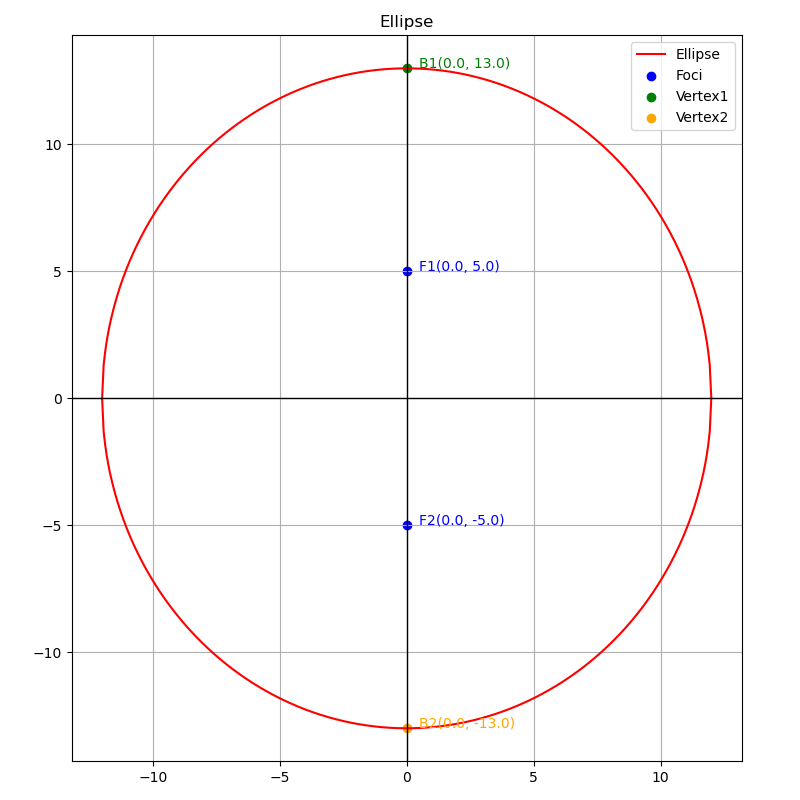
\includegraphics[width=0.6\columnwidth]{figs/ellipse.png} 
   \caption*{Fig : Ellipse}
  \label{Fig1}
\end{figure}

\end{frame}

\end{document}
